\chapter{Introduction}

\begin{figure}[t]
  \begin{center}
  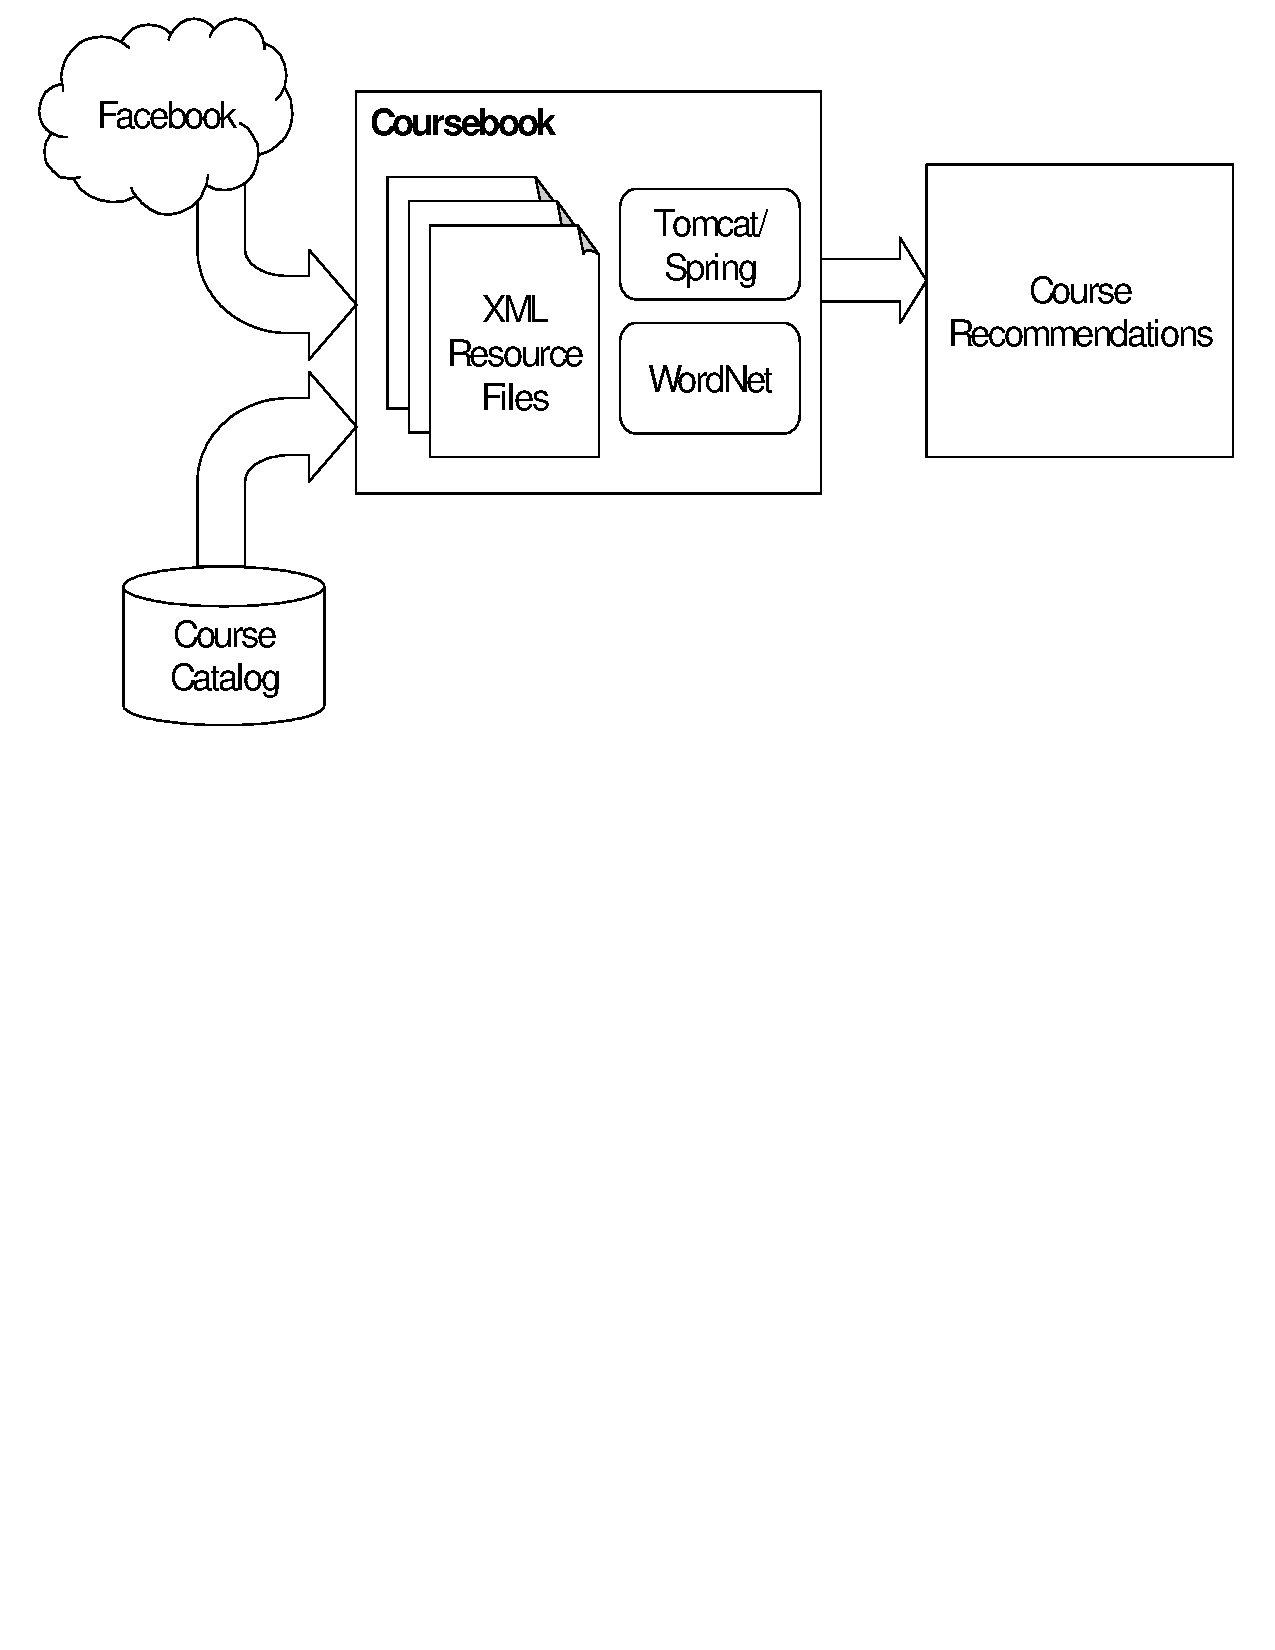
\includegraphics[width=\textwidth]{images/overview}
  \caption{Coursebook Data Flow Overview}
  \label{fig:overview}
  \end{center}
\end{figure}

Facebook is an online social network that allows people to connect with people 
and friends through schools, companies, regions and other groups. Coursebook is
a Facebook enabled website that provides general education course 
recommendations to its users. Coursebook utilizes a relational database of 
course offerings for California Polytechnic State University students to provide
this service. Coursebook is a multi-threaded, highly-concurrent web service 
built on the J2EE platform. By drawing from Facebook's user interests and 
profile information, Coursebook finds which general education classes would be
most appealing to each user. The main task of the system is to provide its users
with relevant general education courses based on their personal interests.

The intended domain is academic, targeting Cal Poly students seeking to enroll 
in general education courses. This gives students an alternative way of finding
general education courses that may interest them, rather than manually searching
through the long list of available classes in the Cal Poly course catalog. 
Coursebook also provides the option of manually entering interests through web
forms to find relevant courses, allowing more flexibility and functionality to
its users. Coursebook aims to provide a service that is:

\singlespacing
\begin{itemize}
  \item easily accessible
  \item highly responsive
  \item fault tolerant
  \item platform agnostic
  \item maintainable for the future
\end{itemize}
\doublespacing

\section{Requirements}

\begin{figure}[t]
  \begin{center}
  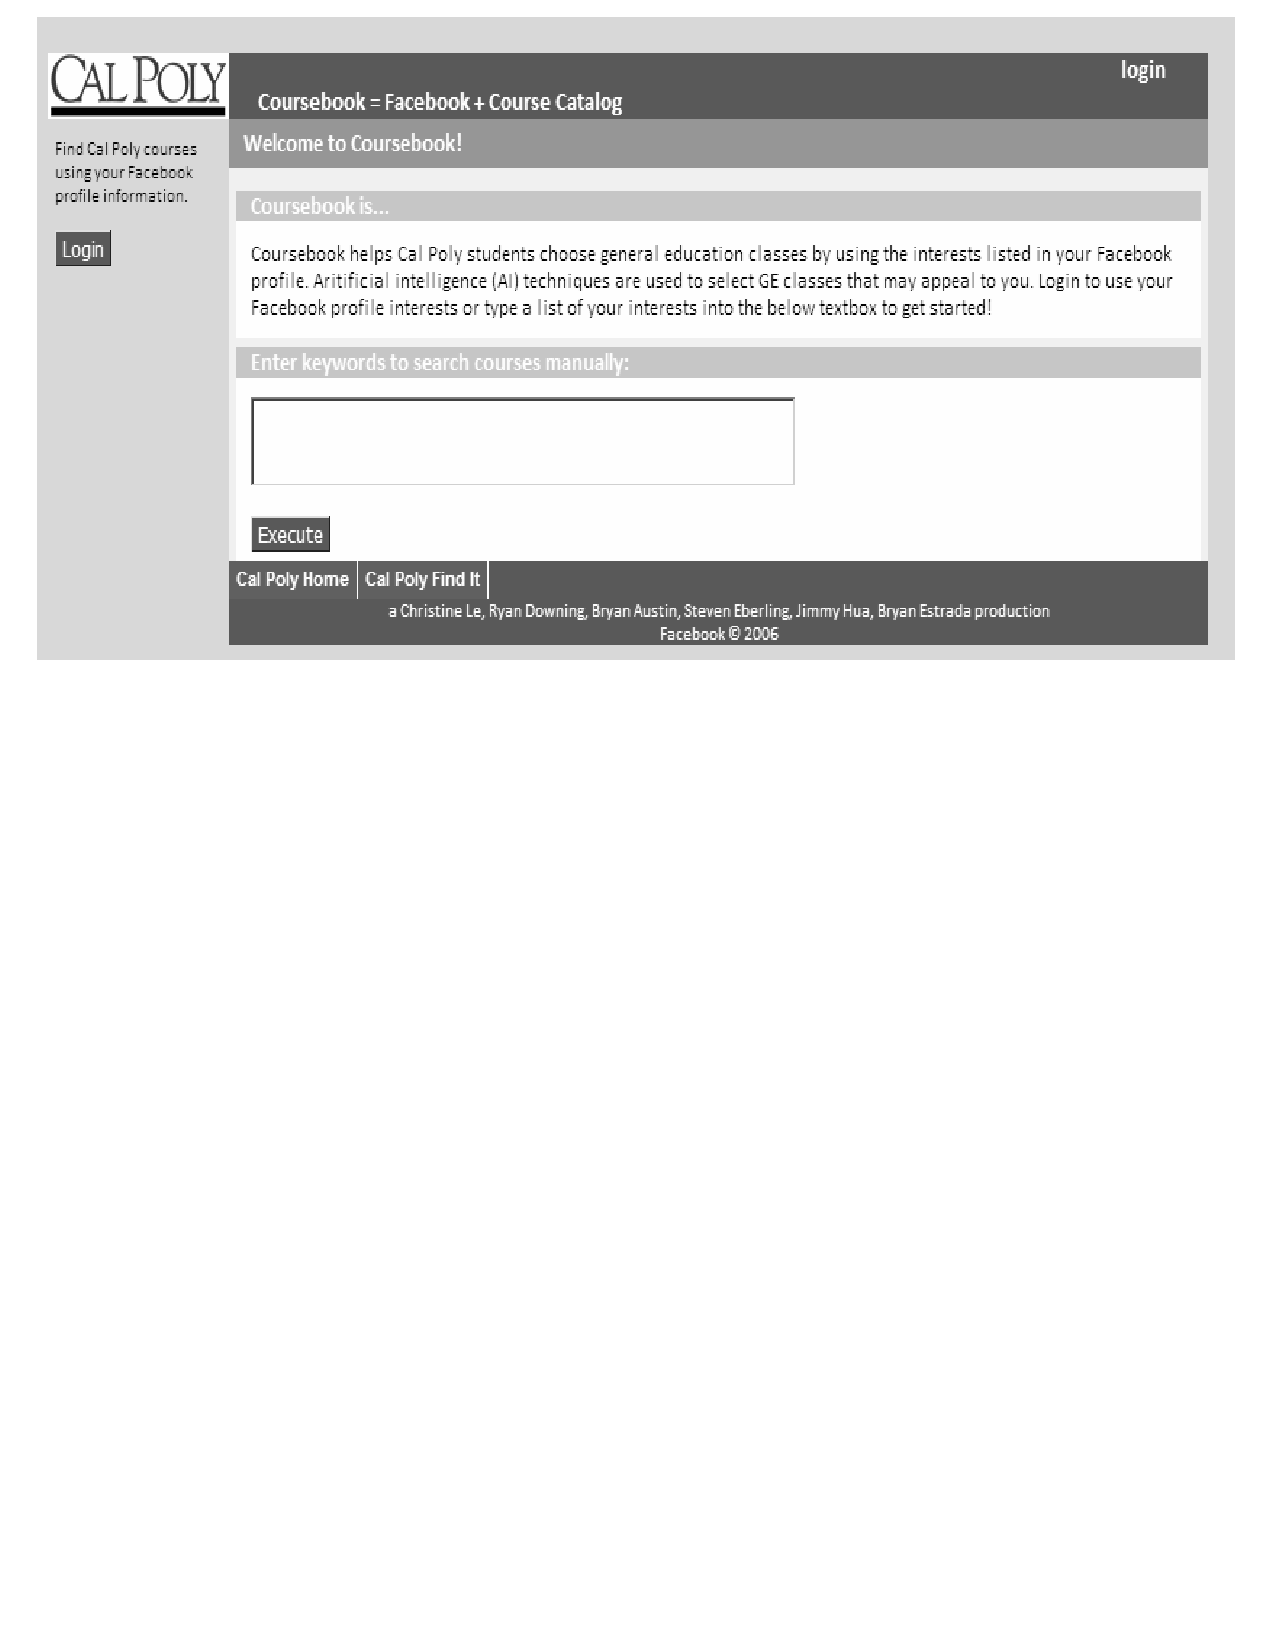
\includegraphics[scale=0.75]{images/screenshot}
  \caption{Coursebook Screenshot}
  \label{fig:screenshot}
  \end{center}
\end{figure}

\subsubsection*{Web User Interface}
By implementing Coursebook with a web-based user interface, we present users 
with an easily accessible service. Coursebook utilizes the latest technologies 
on the J2EE stack, including the Spring framework, JDBC, and WordNet APIs to 
produce a highly responsive system that is platform agnostic on both the server
side (Java) and client side (DHTML/Javascript).

\subsubsection*{Live Data}
Coursebook consists of multiple distributed components to provide users with 
information. The system relies on a MySQL database for real-time course catalog
information. The Facebook API provides developers access to its users' profile 
information. Coursebook offers multiple points of entry, including automatic 
Facebook connectivity and manual user input, in case the former system is 
inaccessible.

\subsubsection*{Relevant Courses}
Coursebook uses advanced artificial intelligence techniques to search and 
compute the most applicable courses for each individual user.

\section{Distributed Components}
\begin{figure}[t]
  \begin{center}
  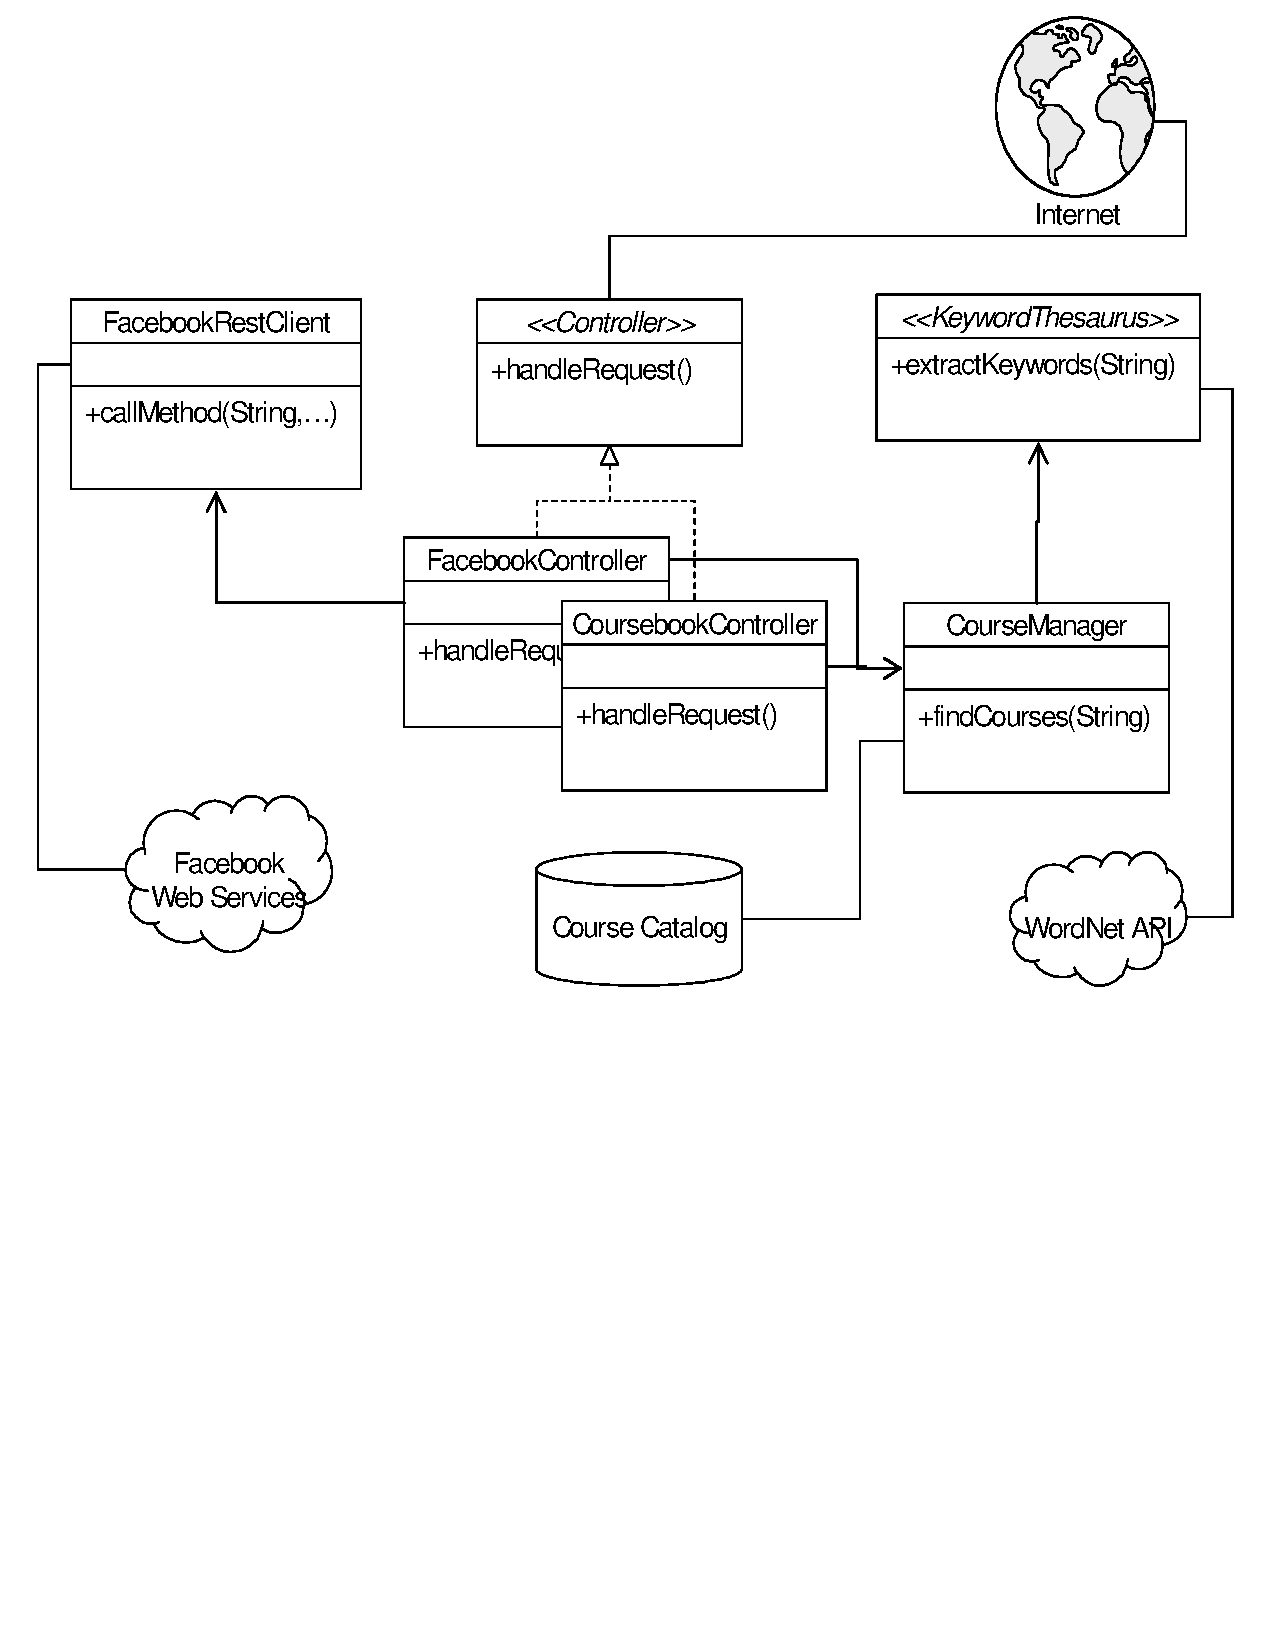
\includegraphics[width=\textwidth]{images/classes}
  \caption{Coursebook Abridged Class Diagram}
  \label{fig:classes}
  \end{center}
\end{figure}


